\documentclass[14 pt]{extarticle}

	\usepackage[frenchb]{babel}
	\usepackage[utf8]{inputenc}  
	\usepackage[T1]{fontenc}
	\usepackage{amssymb}
	\usepackage[mathscr]{euscript}
	\usepackage{stmaryrd}
	\usepackage{amsmath}
	\usepackage{tikz}
	\usepackage[all,cmtip]{xy}
	\usepackage{amsthm}
	\usepackage{varioref}
	\usepackage{geometry}
	\geometry{a4paper}
	\usepackage{lmodern}
	\usepackage{hyperref}
	\usepackage{array}
	 \usepackage{fancyhdr}
	 \usepackage{float}
\renewcommand{\theenumi}{\alph{enumi})}
	\pagestyle{fancy}
	\theoremstyle{plain}
	\fancyfoot[C]{} 
	\fancyhead[L]{Contrôle}
	\fancyhead[R]{13 novembre 2023}\geometry{
 a4paper,
 total={170mm,257mm},
 left=20mm,
 top=20mm,
 }
	
	
	\title{Contrôle Chapitre 2}
	\date{}
	\begin{document}

\begin{center}{\Large Contrôle Chapitre 2}\\ 
 \end{center}
 Nom : \\
 Prénom : \\
 
 \textbf{Tout sur votre copie sauf les exercices 2 et 4.}
 \subsection*{Exercice 1 (4 points)}
Effectuer les calculs suivants : 
\begin{enumerate}
\item $2+ 3 \times 5  $
\item $9\div 3 \times 3$ 
\item $ (2+ 3\times5) \div 2\times 4$
\end{enumerate}


 \subsection*{Exercice 2 (7 points)}
 
 Tracez les symétriques de la figure suivante par rapport à la droite $(d)$ et au point $D$. 
 
 \begin{figure}[H]
 \center
 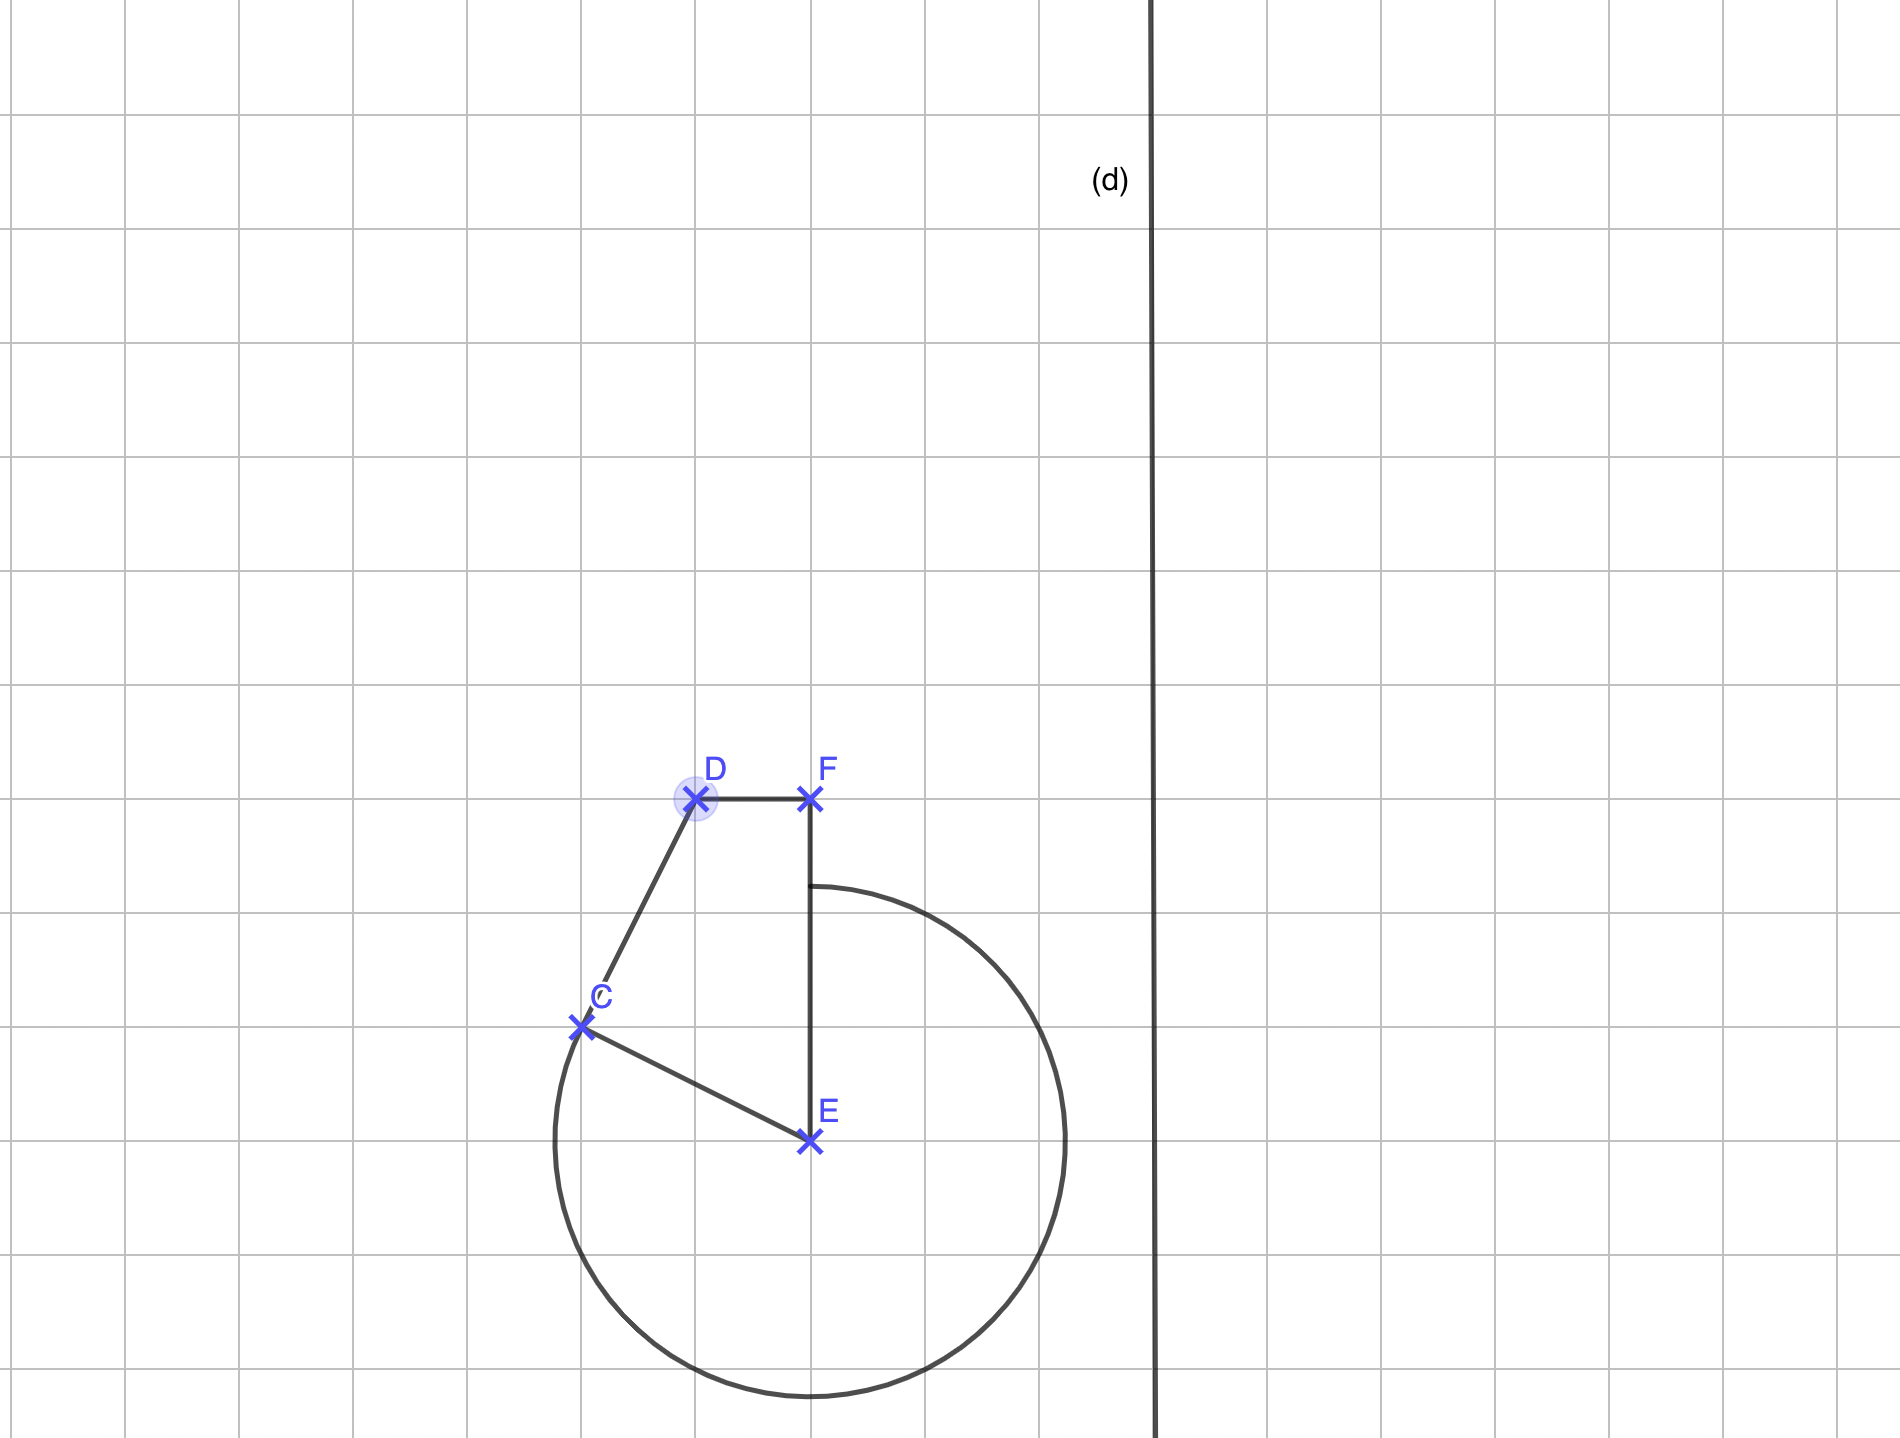
\includegraphics[scale=.55]{Exo1b.png}
 \end{figure}
 
 \subsection*{Exercice 3 (3 points)}
 
 \begin{enumerate}
 \item Tracez un rectangle de côtés $4$ cm et $6$ cm. 
 \item Combien a-t-il d'axes de symétrie ? Tracez-les sur la figure.
 \item A-t-il un centre de symétrie ? Si oui, le représenter sur la
 figure. 
 \end{enumerate}
 
\subsection*{Exercice 4 (3 points)} 

Sur les figures suivantes, représentez les axes et centres de symétrie éventuels, et dites leur nombre.  

\begin{figure}[H]
\center 

\includegraphics[scale=.06]{ecosse.png}\ \ \ \ \ 

\includegraphics[scale=.6]{Blason2.png}\ \ \ \ \ 
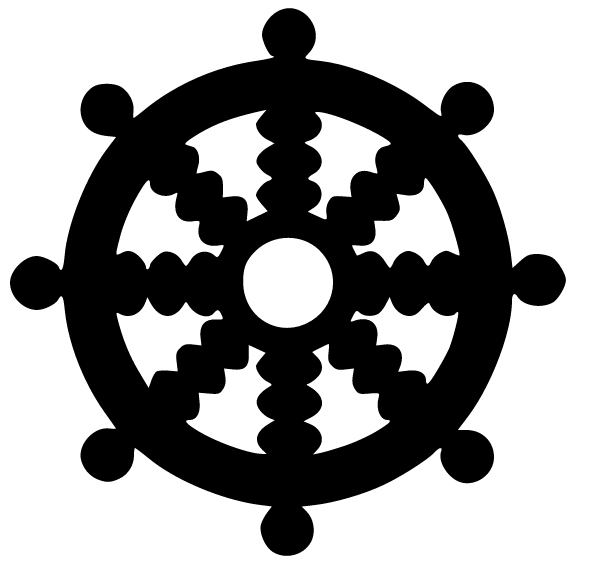
\includegraphics[scale=.4]{Symb2.png}
\end{figure}
 
 \subsection*{Exercice 5 ($3^+$ points)}
 
On veut montrer que les diagonales d'un losange $ABCD$ sont des axes de symétrie. 

\begin{enumerate}
\item Faire une figure à main levée du losange et de ses diagonales. 
\item En utilisant la propriété de la médiatrice, montrer que les points $A$ et $C$ sont sur la médiatrice de $[BD]$. 
\item En déduire que $B$ et $D$ sont symétriques par rapport à $(AC)$. 
\item En déduire que $(AC)$ est un axe de symétrie de la figure $ABCD$. 
\end{enumerate}


\newpage 

\begin{center}{\Large Contrôle Chapitre 2}\\ 
 \end{center}
 Nom : \\
 Prénom : \\
 
 \textbf{Tout sur votre copie sauf les exercices 2 et 4.}
 \subsection*{Exercice 1 (4 points)}
Effectuer les calculs suivants : 
\begin{enumerate}
\item $2+ 7 \times 5  $
\item $8\div 2 \times 2$ 
\item $ (2+ 4\times5) \div 2\times 4$
\end{enumerate}


 \subsection*{Exercice 2 (7 points)}
 
 Tracez les symétriques de la figure suivante par rapport à la droite $(d)$ et au point $D$. 
 
 \begin{figure}[H]
 \center
 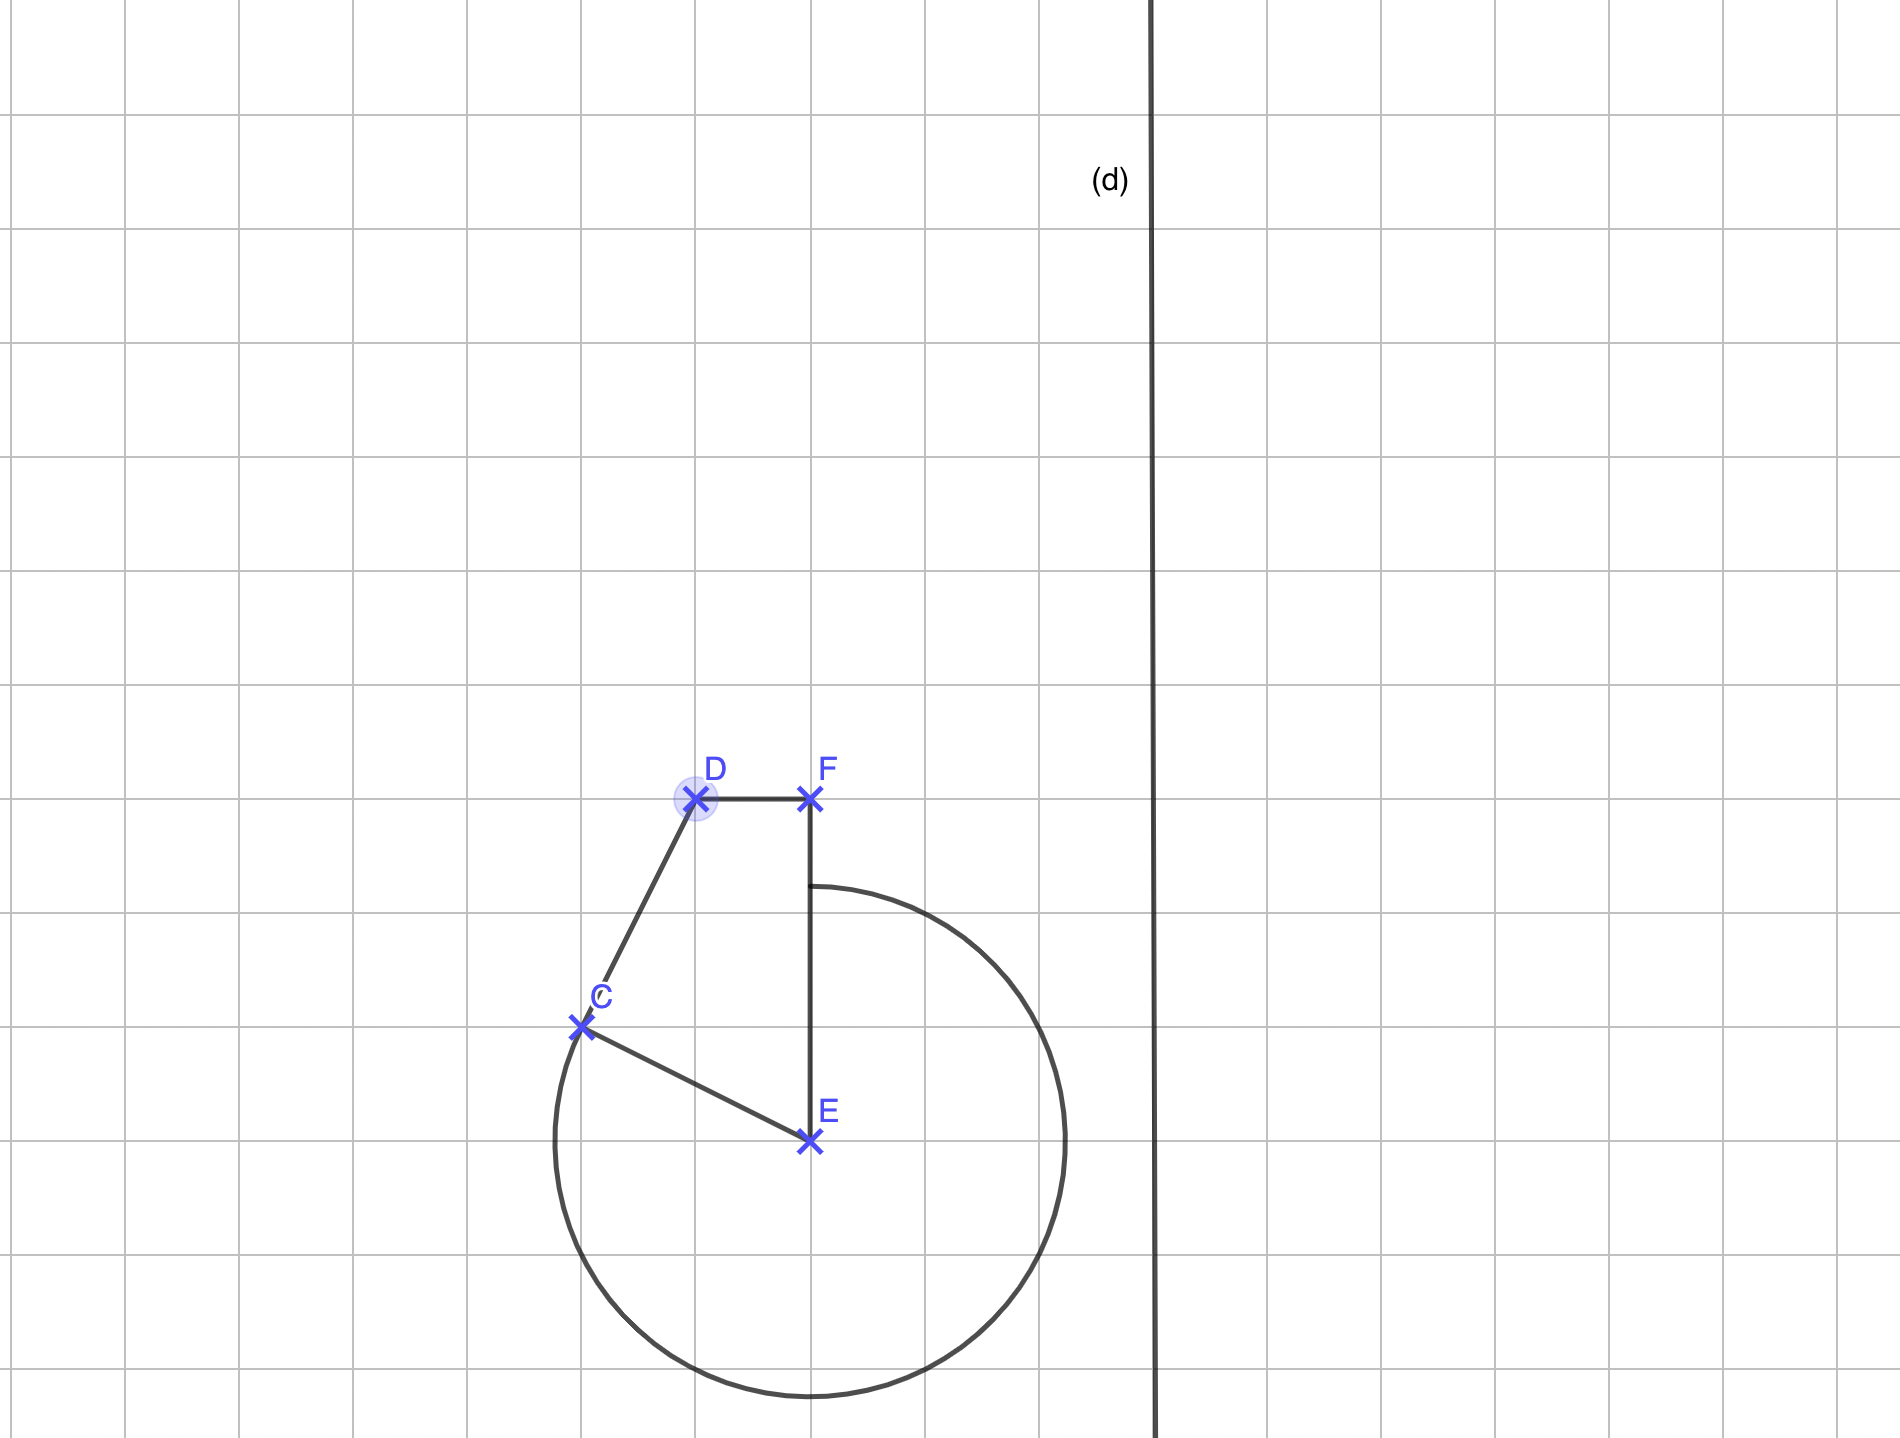
\includegraphics[scale=.5]{Exo1b.png}
 \end{figure}
 
 \subsection*{Exercice 3 (3 points)}
 
 \begin{enumerate}
 \item Tracez un rectangle de côtés $4$ cm et $6$ cm. 
 \item Combien a-t-il d'axes de symétrie ? Tracez-les sur la figure.
 \item A-t-il un centre de symétrie ? Si oui, le représenter sur la
 figure. 
 \end{enumerate}
 
\subsection*{Exercice 4 (3 points)} 

Sur les figures suivantes, représentez les axes et centres de symétrie éventuels, et dites leur nombre.  

\begin{figure}[H]
\center 

\includegraphics[scale=.06]{Grece.png}\ \ \ \ \ 

\includegraphics[scale=.6]{Blason1.png}\ \ \ \ \ 
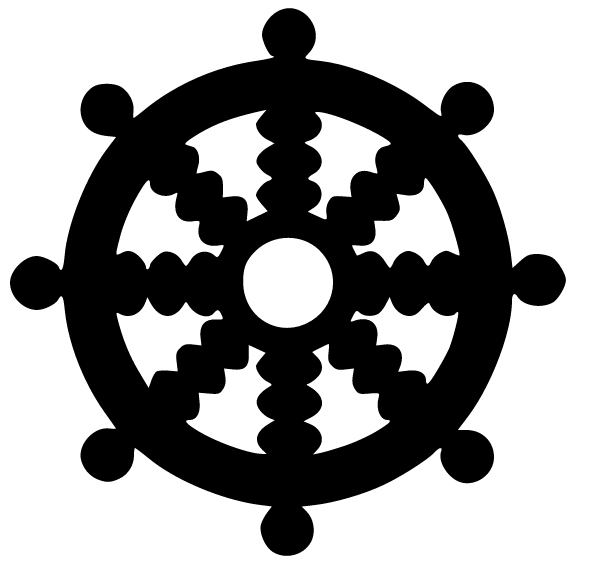
\includegraphics[scale=.4]{Symb2.png}
\end{figure}
 
 \subsection*{Exercice 5 ($3^+$ points)}
 
On veut montrer que les diagonales d'un losange $ABCD$ sont des axes de symétrie. 

\begin{enumerate}
\item Faire une figure à main levée du losange et de ses diagonales. 
\item En utilisant la propriété de la médiatrice, montrer que les points $B$ et $D$ sont sur la médiatrice de $[AC]$. 
\item En déduire que $A$ et $C$ sont symétriques par rapport à $(BD)$. 
\item En déduire que $(BD)$ est un axe de symétrie de la figure $ABCD$. 
\end{enumerate}








 	\end{document}
